\begin{minipage}{0.55\textwidth}
\begin{align*}
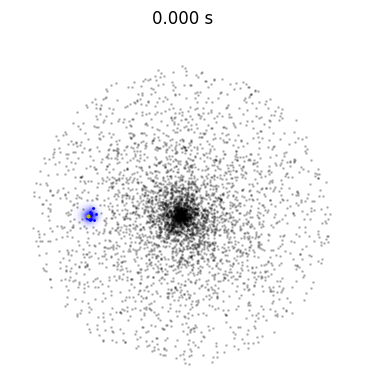
\includegraphics[width=0.49\textwidth]{simulation/6/frame_0.png}\hfill
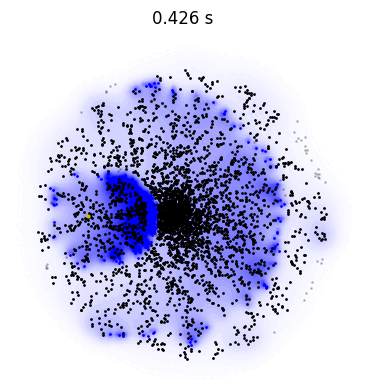
\includegraphics[width=0.49\textwidth]{simulation/6/frame_71.png}
\\[\smallskipamount]
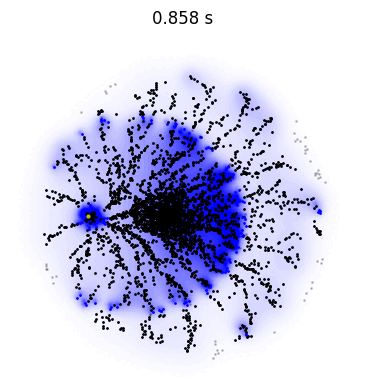
\includegraphics[width=0.49\textwidth]{simulation/6/frame_143.png}\hfill
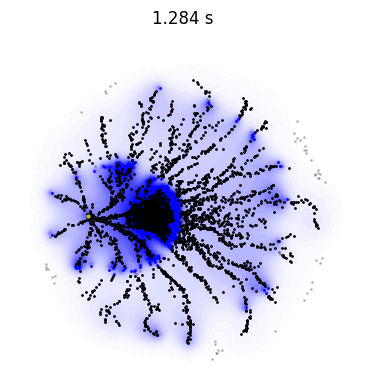
\includegraphics[width=0.49\textwidth]{simulation/6/frame_214.png}
\\[\smallskipamount]
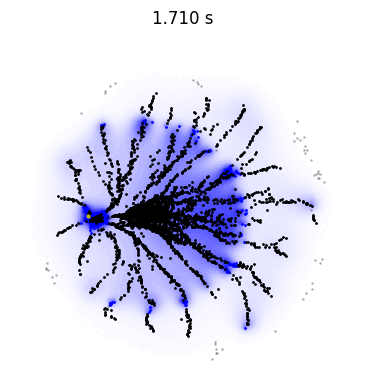
\includegraphics[width=0.49\textwidth]{simulation/6/frame_285.png}\hfill
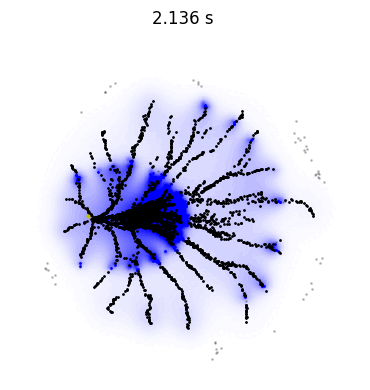
\includegraphics[width=0.49\textwidth]{simulation/6/frame_356.png}
\\[\smallskipamount]
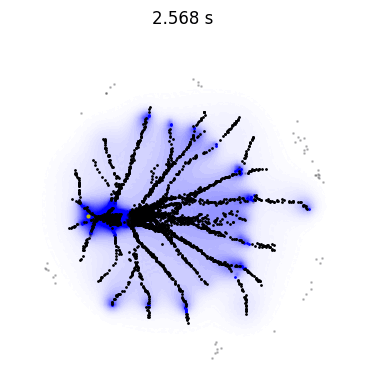
\includegraphics[width=0.49\textwidth]{simulation/6/frame_428.png}\hfill
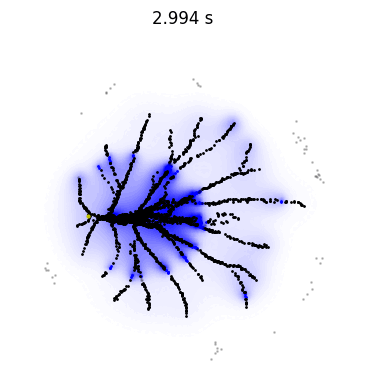
\includegraphics[width=0.49\textwidth]{simulation/6/frame_499.png}
\end{align*}
\end{minipage}
\begin{minipage}{0.45\textwidth}
\subsection{Even Higher Density Center}
Here we use a disk with a even higher density of particles and the dense center still does not seem to affect the spread of the chemical.
However this time the high density area is still present at the end of the simulation as a thick branch.
\end{minipage}